\documentclass{article}

\usepackage[frenchb]{babel}
\usepackage[T1]{fontenc}
\usepackage[utf8]{inputenc}
\usepackage{graphicx}

\title{Manuel d'utilisation de l'application ToDoList}
\author{Anthony Brunel et Antoine Laurent}

\date{\today}

\begin{document}
\maketitle
\newpage

\section{Lancement de l'application}
Pour lancer l'application, il suffit de double cliquer sur ToDoList.jar, de compiler les sources ou bien sous Linux via la commande : \verb+java -jar ToDoList.jar+
\newline
\newline
Une fois l'application lancée on arrive sur la fenêtre principale (Figure~\ref{Fenêtre principale}), c'est à partir de cette fenêtre que l'on va pouvoir gérer nos tâches. 
\newline
Si l'on veut quitter l'application il faut cliquer sur la croix rouge ou bien utiliser la combinaison de touche Alt + f4

\begin{figure}[h]
	\centering
	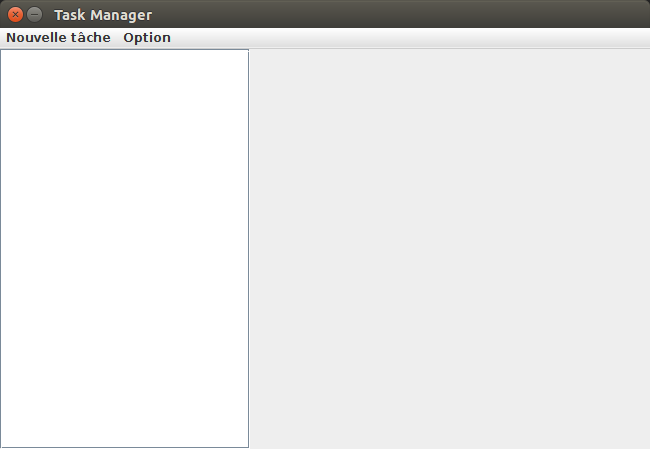
\includegraphics[scale=0.34]{images/MainDIsplay.png}
	\caption{Fenêtre principale}
	\label{Fenêtre principale}
\end{figure}

%\clearpage
\section{Les actions possibles}
Lors de la première utilisation, lorsque vous etes sur la fenêtre principale plusieurs options s'offre alors a vous:
\newline

\begin{itemize}
	\item Créer une tâche au long cours.
	\item Créer une tâche ponctuelle.
	\item Créer ou modifier une catégorie.
	\item Générer le bilan.
	\item Effectuer des tris sur nos tâches.
\end{itemize}

\subsection{Créer une tâche}
Pour créer une tâche il faut appuyer sur le bouton Nouvelle tâche dans le menu (Figure~\ref{Taches barre}), ensuite ous pourrez choisir entre une tâche au long cours ou ponctuelle.

\begin{figure}
	\centering
	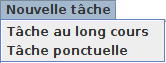
\includegraphics[scale=0.8]{images/MenuTache.png}
	\caption{Ajout d'une tâche}
	\label{Taches barre}
\end{figure}

Une fois choisis il ne vous reste plus qu'à entrer les informations à votre tâche (Figures \ref{Tâche au long cours} et \ref{Tâche Ponctuelle}).

\begin{figure}[!ht]
	\centering
	\begin{minipage}[t]{5cm}
		\centering
		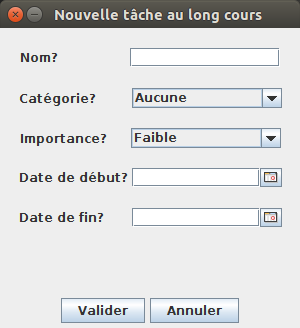
\includegraphics [scale=0.34]{images/NewTAsk1.png}
		\caption{Tâche au long cours}
		\label{Tâche au long cours}
	\end{minipage}
	\begin{minipage}[t]{5cm}
		\centering
		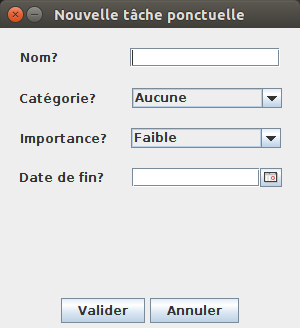
\includegraphics [scale=0.34]{images/NewTAsk2.png}
		\caption {Tâche Ponctuelle}
		\label{Tâche Ponctuelle}
	\end{minipage}
\end{figure}

\textbf{NB :} vous pouvez soit rentrer les dates soit les choisirs avec le calendrier.
\newline
\newline
Lorsque l'on ajoute une tâche, on retourne sur la fenêtre principale, les tâches au long cours apparaîtront bleues et les tâches ponctuelles vertes. Le nombre de jours restant avant la fin de la tâche sera indiqué à coté de celle-ci.
De plus, si une tâche est en retard un petit panneau rouge vous l'indiquera.(Figure \ref{Fenetre principale 2}).

\begin{figure}[!h]
	\centering
	\includegraphics[scale=0.34]{images/CaptureMainDIsplay3.png}
	\caption{Fenetre Principale avec tâches}
	\label{Fenetre principale 2}
\end{figure}

\clearpage
\subsection{Créer Modifier une catégoire}
Pour créer/modifier une catégorie il suffit de cliquer sur Option puis Catégorie (Figure \ref{barre Opiton}).

\begin{figure}[h]
	\centering
	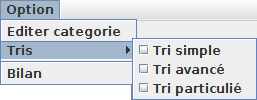
\includegraphics[scale=0.6]{images/MenuOption.png}
	\caption{Menu Option}
	\label{barre Opiton}
\end{figure}

Ensuite vous pouvez voir toutes les catégories, en modifier, en ajouter et en supprimer (Figure \ref{modif Opiton}).

\begin{figure}[h]
	\centering
	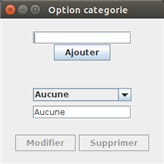
\includegraphics[scale=0.8]{images/Capture_edit_categorie.jpg}
	\caption{Modification d'une Catégorie}
	\label{modif Opiton}
\end{figure}

%\clearpage
\subsection{Générer le bilan}

Notre application permet aussi de générer le bilan, pour ceci il faut cliqué sur le bouton Option puis bilan (Figure \ref{barre Opiton}).
Une nouvelle fenêtre s'ouvre ou il faut rentré la date de début et la date de fin de la période sur laquelle on veut générer le bilan et cliquer sur "générer" (Figrue \ref{bilan}).

\begin{figure}
	\centering
	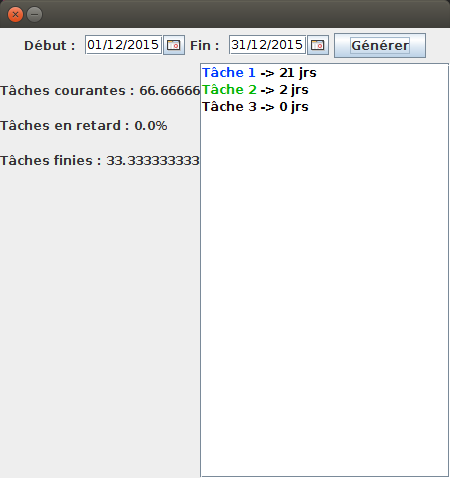
\includegraphics[scale=0.4]{images/CaptureDisplayBilan.png}
	\caption{Fenêtre bilan}
	\label{bilan}
\end{figure}

La fenêtre contiendra les taches comprise dans le bilan, leur status (les tâches finies sont en noir les autres sont en couleur), et le pourcentages de tâches courantes, en retard et finies sur cette période.

\subsection{Les tris}

Il y a trois tris a disposition, le lris simple (tris par deadline), le tris avancé (tris en fonction des échéances intermédiaires), pour les activés il faut cliquer sur option puis sélectioner le tris souhaité (Figure \ref{barre Opiton}).

\end{document}
